%%%%%%%%%%%%%%%%%%%%%%%%%%%%%%%%%%%%%%%%%%%%%%%%%%%%%%%%%%%%%%%%%%%%%%%
%% template for II2202 report
%% original 2015.11.24
%% revised  2018.08.26
%%%%%%%%%%%%%%%%%%%%%%%%%%%%%%%%%%%%%%%%%%%%%%%%%%%%%%%%%%%%%%%%%%%%%%%
%

\title{GPU Dynamic memory allocation algorithms for Machine Learning: A survey}
\author{
        \textsc{Erik H. Wouters}
            \qquad
        \textsc{Dragos S. Perju}
        \mbox{}\\
        \normalsize
            \texttt{ehwo}
        \textbar{}
            \texttt{dsperju}
        \normalsize
            \texttt{@kth.se}
}
\date{\today}

\documentclass[12pt,twoside]{article}

\usepackage[paper=a4paper,dvips,top=1.5cm,left=1.5cm,right=1.5cm,
    foot=1cm,bottom=1.5cm]{geometry}
\usepackage[disable]{todonotes}

%\usepackage[T1]{fontenc}
%%\usepackage{pslatex}
\renewcommand{\rmdefault}{ptm} 
\usepackage{mathptmx}
\usepackage[scaled=.90]{helvet}
\usepackage{courier}
%
\usepackage{bookmark}

\usepackage{fancyhdr}
\pagestyle{fancy}

\usepackage{nameref}

%%----------------------------------------------------------------------------
%%   pcap2tex stuff
%%----------------------------------------------------------------------------
 \usepackage[dvipsnames*,svgnames]{xcolor} %% For extended colors
 \usepackage{tikz}
 \usetikzlibrary{arrows,decorations.pathmorphing,backgrounds,fit,positioning,calc,shapes}

%% \usepackage{pgfmath}	% --math engine
%%----------------------------------------------------------------------------
%% \usepackage[latin1]{inputenc}
\usepackage[utf8]{inputenc} % inputenc allows the user to input accented characters directly from the keyboard
\usepackage[swedish,english]{babel}
%% \usepackage{rotating}		 %% For text rotating
\usepackage{array}			 %% For table wrapping
\usepackage{graphicx}	                 %% Support for images
\usepackage{float}			 %% Suppor for more flexible floating box positioning
\usepackage{color}                       %% Support for colour 
\usepackage{mdwlist}
%% \usepackage{setspace}                 %% For fine-grained control over line spacing
%% \usepackage{listings}		 %% For source code listing
%% \usepackage{bytefield}                %% For packet drawings
\usepackage{tabularx}		         %% For simple table stretching
%%\usepackage{multirow}	                 %% Support for multirow colums in tables
\usepackage{dcolumn}	                 %% Support for decimal point alignment in tables
\usepackage{url}	                 %% Support for breaking URLs
\usepackage[perpage,para,symbol]{footmisc} %% use symbols to ``number'' footnotes and reset which symbol is used first on each page

%% \usepackage{pygmentize}           %% required to use minted -- see python-pygments - Pygments is a Syntax Highlighting Package written in Python
%% \usepackage{minted}		     %% For source code highlighting

%% \usepackage{hyperref}		
\usepackage[all]{hypcap}	 %% Prevents an issue related to hyperref and caption linking
%% setup hyperref to use the darkblue color on links
%% \hypersetup{colorlinks,breaklinks,
%%             linkcolor=darkblue,urlcolor=darkblue,
%%             anchorcolor=darkblue,citecolor=darkblue}

%% Some definitions of used colors
\definecolor{darkblue}{rgb}{0.0,0.0,0.3} %% define a color called darkblue
\definecolor{darkred}{rgb}{0.4,0.0,0.0}
\definecolor{red}{rgb}{0.7,0.0,0.0}
\definecolor{lightgrey}{rgb}{0.8,0.8,0.8} 
\definecolor{grey}{rgb}{0.6,0.6,0.6}
\definecolor{darkgrey}{rgb}{0.4,0.4,0.4}
%% Reduce hyphenation as much as possible
\hyphenpenalty=15000 
\tolerance=1000

%% useful redefinitions to use with tables
\newcommand{\rr}{\raggedright} %% raggedright command redefinition
\newcommand{\rl}{\raggedleft} %% raggedleft command redefinition
\newcommand{\tn}{\tabularnewline} %% tabularnewline command redefinition

%% definition of new command for bytefield package
\newcommand{\colorbitbox}[3]{%
	\rlap{\bitbox{#2}{\color{#1}\rule{\width}{\height}}}%
	\bitbox{#2}{#3}}

%% command to ease switching to red color text
\newcommand{\red}{\color{red}}
%%redefinition of paragraph command to insert a breakline after it
\makeatletter
\renewcommand\paragraph{\@startsection{paragraph}{4}{\z@}%
  {-3.25ex\@plus -1ex \@minus -.2ex}%
  {1.5ex \@plus .2ex}%
  {\normalfont\normalsize\bfseries}}
\makeatother

%%redefinition of subparagraph command to insert a breakline after it
\makeatletter
\renewcommand\subparagraph{\@startsection{subparagraph}{5}{\z@}%
  {-3.25ex\@plus -1ex \@minus -.2ex}%
  {1.5ex \@plus .2ex}%
  {\normalfont\normalsize\bfseries}}
\makeatother

%% DP: making \todo[inline] actually on the same line as a paragraph
\makeatletter 
\tikzstyle{inlinenotestyle} = [
    draw=\@todonotes@currentbordercolor,
    fill=\@todonotes@currentbackgroundcolor,
    line width=0.5pt,
    inner sep = 0.8 ex,
    rounded corners=4pt]

\renewcommand{\@todonotes@drawInlineNote}{%
        {\begin{tikzpicture}[remember picture,baseline=(current bounding box.base)]%
            \draw node[inlinenotestyle,font=\@todonotes@sizecommand, anchor=base,baseline]{%
              \if@todonotes@authorgiven%
                {\noindent \@todonotes@sizecommand \@todonotes@author:\,\@todonotes@text}%
              \else%
                {\noindent \@todonotes@sizecommand \@todonotes@text}%
              \fi};%
           \end{tikzpicture}}}%
\newcommand{\mytodo}[1]{\@todo[inline]{#1}}%
\makeatother

\setcounter{tocdepth}{3}	%% 3 depth levels in TOC
\setcounter{secnumdepth}{5}


\newcommand{\resnettimebfc}{$5.82$}
\newcommand{\resnettimecuda}{$5.32$}
\newcommand{\resnettimehalloc}{$?$}
\newcommand{\alexnettimebfc}{$41.71$}
\newcommand{\alexnettimecuda}{$40.24$}
\newcommand{\alexnettimehalloc}{$?$}

%%%%%%%%%%%%%%%%%%%%%%%%%%%%%%%%%%%%%%%%%%%%%%%%%%%%%%%%%%%%%%%%%%%%
%% End of preamble
%%%%%%%%%%%%%%%%%%%%%%%%%%%%%%%%%%%%%%%%%%%%%%%%%%%%%%%%%%%%%%%%%%%%

\renewcommand{\headrulewidth}{0pt}
\lhead{II2202, Fall 2018, Period 1-2}
%% or \lhead{II2202, Fall 2016, Period 1}
\chead{Draft project report}
\rhead{\date{\today}}

\makeatletter
\let\ps@plain\ps@fancy 
\makeatother

\setlength{\headheight}{15pt}
\begin{document}

\maketitle


\begin{abstract}
\label{sec:abstract}

We compare 4 dynamic memory allocators designed for running on GPUs and select the best performing under TensorFlow’s Convolutional Neural Network (CNN) benchmark, running only the ResNet-50 model. Our main metric of comparison is the number of images per second processed by the benchmark. Other metrics studied are: object sizes requested for allocation by the benchmark and the frequency in allocation request and in the sizes used. After our performance analysis, we conclude that \texttt{Halloc} algorithm is better than the already used algorithms by TensorFlow, \texttt{CUDAMalloc} and \texttt{BFCMalloc}, in the context of the benchmark itself.\footnote{Not proven yet. Might possibly also be false.}.

\textbf{Keywords:} Algorithm, Performance, Machine learning, GPU, Dynamic memory, Allocation, TensorFlow

\end{abstract}
%%\clearpage

\selectlanguage{english}
\tableofcontents

\section*{List of Acronyms and Abbreviations}
\label{list-of-acronyms-and-abbreviations}

This document requires readers to be familiar with terms and concepts described in \mbox{RFC~1235} \cite{john_ioannidis_coherent_1991}. For clarity we summarize some of these terms and give a short description of them before presenting them in next sections.

\begin{basedescript}{\desclabelstyle{\pushlabel}\desclabelwidth{10em}}
\item[CNN]					Convolutional Neural Network \cite{postel_internet_1981})
\item[CPU]                  Central Processing Unit
\item[GPU]                  Graphics Processing Unit
\item[ML]                   Machine Learning
\item[SIMD]                 Single-Instruction Multiple-Data
\item[CUDA]                 Compute Unified Device Architecture
\end{basedescript}


\clearpage


\todo[inline]{Change \textbackslash usepackage\{todonotes\}\ to\ \textbackslash usepackage[disable]\{todonotes\} to hide the todo notes}

\todo[inline]{as we'll probably not finish them all by Friday.}

\section{Introduction}
\label{sec:introduction}
%% Longer problem statement
%% General introduction to the area

% See also \cite{a_new_synchronization_protocol_for_sqlite_databases},
% the paper \cite{anand_kannan_n-ary_2012}, 
% and the book \cite{brent_s._baxter_standard_1982}.

%Many examples of real-life scenarios show how machine learning directly impacts people's day-to-day lives, such as in the application domains of: smart farming\todo[inline]{[1 TODO]}, city vehicle traffic\todo[inline]{[2 TODO]}, video surveillance and so on. 

%It is therefore important to improve such complex computer techniques, by improving the basic computer algorithms on which these advanced techniques are based upon. One such basic technique is dynamic memory allocation.

Machine learning represents a major and computationally intensive computing technique that is one of the most important drivers of progress of humankind and of the technology we use today. We aim to raise the performance of such a complex programming technique by catering to one of the basic computing techniques it uses: dynamic memory allocation on graphics processing unit (GPU).

% by interchanging with the ones that are already implemented in the well-known machine learning (ML) software library TensorFlow. 

In the present research paper, we offer a comparison of the performance of several dynamic memory allocation algorithms running on the GPU, executed by a benchmark of the well-known machine learning (ML) software library TensorFlow. The benchmark constructs Convolutional Neural Networks (CNN) of different models: ResNet-50, AlexNet.

Different dynamic memory allocation algorithms capable to run on the GPU are selected and studied based on different factors (such as \textit{speed}, \textit{memory management} and \textit{object sizes} requested for allocation). The algorithms chosen are: \texttt{CUDAMalloc} (or \texttt{cuMalloc}), \texttt{BFCMalloc} and \texttt{Halloc}.

Descriptions of TensorFlow, the benchmark, the CNN models that are studied, the dynamic memory allocation algorithms and possible issues with dynamic memory allocation in general are under the sub-section \textit{\nameref{sec:theoretical-framework}} of this \textit{\nameref{sec:introduction}} section. In section \ref{sec:questions}, \textit{\nameref{sec:questions}}, it is laid out the conclusions we want to make and our expectations of the results, before running the benchmark. Most algorithms come accompanied with their own descriptions that offer an idea in which situations such algorithms would behave better than in other situations. Section \ref{sec:methods}, \textit{\nameref{sec:methods}}, includes the system configuration on which the the tests were executed, as well as the description of the test paradigm this study entails. Section \ref{sec:results-and-analysis}, \textit{\nameref{sec:results-and-analysis}} includes the final graphs and tables with data after an extensive run of our tests. Here, we also discuss the different aspects that such results entail: there's no one allocator that satisfies all supposed requirements. Finally, under the section \ref{sec:discussion}, \textit{\nameref{sec:discussion}}, we draw a conclusion for what allocators are the best in which cases.




\subsection{Theoretical framework}
\label{sec:theoretical-framework}

\subsubsection*{TensorFlow}

TensorFlow is an open-source software library that can perform numerical computation using data flow graphs. It can therefore perform machine learning in a faster and easier manner, being one of its main application purposes. TensorFlow was developed and used in-house by a research team at Google, being released afterwards to the public on November 2015 on GitHub. The very first public version of TensorFlow contains parts of another deep learning project named Caffe, developed at University of California, having a copyright notice alongside, dated 2014.

Yet, ever since TensorFlow was developed, its main dynamic memory allocation algorithm for GPU use is the \texttt{BFCAllocator}. In its own source code, \texttt{BFCAllocator} is described to be: \textit{a memory allocator that implements a 'best-fit with coalescing' algorithm.  [...] [It] is essentially a very simple version of Doug Lea's malloc (dlmalloc) \cite{dlmalloc}}.

CUDA's own dynamic memory allocator, \texttt{cuMalloc}, is kept as an easy selectable alternative, before running TensorFlow. It is however composed of proprietary code and does not share anything else but the header file that only allows it to be used. As such, we cannot investigate the code to see what type of allocator this is. However, \citeauthor{Vinkler2015} states that \texttt{cuMalloc} is relatively slow for allocations of small sized objects \cite{Vinkler2015}.
% As such, we cannot say what type of allocator \texttt{cuMalloc} is -- as different allocator algorithms can be categorized in different types.

\subsubsection*{Dynamic memory allocation}

Dynamic memory allocation is a technique well-known and often used by programmers. Much of the work for improvement and research on this topic is being devoted to the context of single-core and multi-core general purpose processors \cite{YOU2015}. In comparison to static memory allocation, which happens at program compilation time and is more frequently used in programming, dynamic memory allocation brings along issues with its use, such as fragmentation and memory leaks \cite{TRAISTER199099}.

Such problems make dynamic memory allocation algorithms unsuitable for use on specific platforms, such as safety-critical embedded systems \cite{Puaut_2002}. The technique however did progress to be implemented on systems other than GPUs. GPUs introduce new difficulties in implementing dynamic memory allocation, being many-core systems running many more threads, distributed on many more cores than general purpose processors usually have. GPUs however evolved to be used for more than just rendering images, being used for complex programming techniques such as \textit{machine learning}. This makes dynamic memory allocation important in the context of GPUs, in order to attain efficiency for such applications.

Literature:
\url{https://devtalk.nvidia.com/default/topic/878664/custom-memory-allocator-for-cuda-desired/}
\url{https://riptutorial.com/TensorFlow/example/13427/use-the-tcmalloc-allocator}
\url{http://on-demand.gputechconf.com/gtc/2014/presentations/S4271-halloc-high-throughput-dynamic-memory-allocator.pdf}

%Different programming languages offer different ways of managing variables. Most of them use a dynamic memory allocation algorithm. This algorithm returns a memory address when request to create a new variable is executed. In higher level programming languages there is no direct interaction with the memory addresses, but in lower level languages programmers can employ advanced techniques to manage the memory more efficiently for a specific application \cite{TRAISTER199099}.

\subsection{Research questions}
\label{sec:questions}

\subsusection{Problem Statement}
\label{sec:problem-statement}

%\todo{Describe the problem(s) that have been found in the area described in the background. Describe the problem area (in detail). For example:}

% \textbf{\textit{Maybe this book can be cited somewhere:}} \cite{GINSBURG2017345} \\

CUDA offers, to programmers who want to take advantage of GPU's processing power, a proprietary, unpublished algorithm for dynamically allocating memory called \texttt{CudaMalloc}. However, dynamic memory allocation algorithms running on the CPU are often customized for certain programs that require the edge in speed or stability, such as video games, database engines and so on. It is only natural to suspect that Machine Learning algorithms would be able to deliver faster performances if an allocator tailored for their needs would be selected as well.

We believe that \texttt{CudaMalloc}, as a general purpose dynamic memory allocation algorithm for the GPU, can be replaced for better performances when using the TensorFlow \cite{abadi2016} library for Machine Learning processing. In particular the ResNet-50 implementation of TensorFlow will be evaluated, which is a Convolutional Neural Network (CNN) with many layers and will therefore allocate many small sized objects in the GPU memory \cite{DBLP:HeZRS15}.
Algorithms that possibly perform better are mentioned in the work of \citeauthor{Vinkler2015} \cite{Vinkler2015}. They state that \texttt{CudaMalloc} is slower to process than other allocation algorithms for allocating many small sized objects, as shown in Figure 3a in \cite{Vinkler2015}. We decide to therefore select the better allocation algorithm for the task at hand, through the proposed research.

\subsection{Problem}
\label{sec:problem}

%\todo{State a clear and concise problem that is going to be investigated.  Answer the question What is the real problem? - What is the problem or value proposition addressed by the project? – Ideally one sentence that is very concrete. For example:}

%Fast Machine Learning processing imposes specific constraints of the dynamic memory allocator that runs on the GPU, 

The memory allocation pattern of TensorFlow's implementation of ResNet-50 is not a great match for the memory allocator TensorFlow uses, we will investigate which previously published dynamic memory allocation algorithms perform better.

%The need for fast Machine Learning processing, by improving the dynamic memory allocation that runs on the GPU.

%Select the fastest, state of the art, open source GPU dynamic memory allocation algorithm for a Machine Learning workload.

\subsection{Hypothesis}
\label{sec:hypothesis}

%\todo{State a hypothesis that you think would be the outcome of your investigation. Answer the question: What is your hypothesis? (Note that the hypothesis must be measurable to be confirmed or falsified. Moreover not all projects have hypothesis.).}

Our hypothesis is that one or more of the algorithms described by \citeauthor{Vinkler2015} \cite{Vinkler2015} perform better as a memory allocator for TensorFlow's implementation of \texttt{ResNet-50} than the stock \texttt{BFCAllocator} or the standard \texttt{CudaMalloc} does, in terms of overall speed, fragmentation and stability.

%when allocation requests vary in size or frequency (consecutive or varied requests).

\subsection{Purpose}
\label{sec:purpose}

%\todo{Explain the purpose(s) of your project / investigation (the expected deliverables from the project). Answer the question: Why do this project? (purpose/effect, i.e. – the purpose can be to save environment but the goal is to build a robot that can pick up trash.) Why would you carry out the project? For example:}

Machine Learning is a technology that helps with the advancement on many problems we are struggling with today. From drug discovery \cite{Ramsundar_Kearnes_Riley_Webster_Konerding_Pande_2015} to sorting cucumbers by quality \cite{cucumber}, Machine Learning has applications in domains such as medical, agricultural, security, marketing and many others. It is through the presented project that we want to contribute to the progress of a programming tool that betters the lives of people.

\subsection{Goal(s)}
\label{sec:goal(s)}

%\todo{Explain the goal(s), objective(s), and/or the result(s) of your investigation. What are the expected deliverables/outcomes from the project? For example:}

1. Design a repeatable experiment that shows that one of the GPU memory allocation algorithms presented by \citeauthor{Vinkler2015} \cite{Vinkler2015} is faster than the standard \texttt{CudaMalloc} function. This experiment will be used to validate the hypothesis. 2. Understand why this algorithm is faster (or slower).
If we find a faster algorithm, send results and recommendation to the TensorFlow team for study and possible implementation in the release version.


\section{Methods}
\label{sec:methods}

%\todo{Describe and explain the research methods that will be used for the project. What research method (or methods) will be used? Argue: why this is the most appropriate method or methods. For example:}

\begin{itemize}
\vspace{-10px}
\itemsep-0.25em 
\item the speed (measured in \textit{images/second});
\item the reliability of the allocators as the size of the model is raised (does the allocator not have enough memory at some point, due to poor memory management?);
\item the frequency in size of the objects requested to be allocated, as some allocators may prove to run better if most allocated objects are smaller or bigger.
\vspace{-10px}
\end{itemize}

We decide to tackle allocation algorithms running on GPUs because machine learning takes advantage of their multiple core setup, threading capabilities and single-instruction multiple-data (SIMD) type of computation, achieving more than average performance than running on general purpose processors. TensorFlow already implements \texttt{CUDAMalloc} and \texttt{BFCMalloc} as its two selectable options for GPU method of allocation, with the latter being the default. In our initial comparison, \texttt{CUDAMalloc} achieves ${\sim}\resnettimecuda$ images/second performance when running the ResNet-50 benchmark, while BFCMalloc attains ${\sim}\resnettimebfc$ images/second, showing that, in fact, dynamic memory allocation algorithms can have an impact on the overall performance of machine learning software.

Our main metric for comparison is, indeed, the speed of the construction of the ResNet-50 model that the benchmark can attain, expressed in \textit{images/second}. It is the main output that the benchmark shows while executing. Additionally, we study the object sizes being allocated throughout the runtime of the benchmark, in order to discuss why some allocators can perform better or worse for certain object sizes are requested for allocation. Furthermore, we consider of interest to change the model sizes wanted to be constructed by the benchmark, as some allocators can prove to be better with memory management than with other factors, successfully obtaining bigger models than its counterparts -- which could interrupt inadvertently when required to construct bigger models.\todo[inline]{We could also try other models}

- Argue that memory map is quite unuseful

-  we inject the code to provide output information of the sizes of objectes requested for allocation by the benchmark. In such a way, we know w

Focusing on such a metric means we maintain the 

- Also, we deem of interest to try out different model sizes, in order to see not only the speed of certain allocation algorithms, but how well they manage the memory throughout the benchmark run, possibly running slower in general but are able to construct a bigger model fully than its counterparts, which can interrupt unwantingly mid-way.


We will compile TensorFlow on Erik Wouters' HP ZBook workstation laptop (equipped with an NVIDIA K1100M GPU) and run the TensorFlow Convolutional Neural Network benchmarks from \url{https://github.com/TensorFlow/benchmarks}. To compare the different memory algorithms, we will repeat the compilation and benchmarking with a subset of the memory allocation algorithms described by \citeauthor{Vinkler2015} \cite{Vinkler2015}.

The project will use the empirical method \cite{bock2001}. As we are evaluating using a well known benchmark from the Machine Learning field, this will provide results that mimic real world performance of these algorithms applied to Machine Learning \cite{abadi2016}. In order to create results that are as repeatable as possible, each test will be run 5 times and then the times will be averaged together. The NVIDIA K1100M GPU will run in it's default state on Erik Wouters' HP ZBook. For each test, 10 warm-up steps will be done and then the next 100 steps will be averaged. 

Replication information:
\begin{itemize}
    \item Bazel 0.18.1
    \item CUDA 9.0
    \item cuDNN 7.0.5 (we must mention 7.0.5 vs 7.4 is 3 times slow \url{https://developer.nvidia.com/sites/default/files/akamai/deeplearning/cudnn/cudnn_7.4_cnn_1.png})
    \item gcc 6.4.0 (symlinked to /usr/bin/gcc)
    \item Ubuntu 18.04 LTS (4.15.0-39-generic)
    \item TensorFlow v1.11.0
    \item Python 3.5.6 Anaconda
    \item Halloc 0.11
\end{itemize}


\todo[inline]{Notes about how bazel sucks.}


\section{Results and Analysis}
\label{sec:results-and-analysis}

In our initial comparisons, we have found TensorFlow's default allocator, BFCAllocator, to attain ~8 images per second when processing the ResNet-50 model benchmark, while \texttt{cuMalloc} attains only ~5.3 images per second. This proves that there is significance in such a research, as choosing the right dynamic memory allocator can have a large impact on the performance of high end algorithms and computing techniques.

The initial benchmarks are shown in table \ref{tab:results}. The images/sec column shows the average amount of images that are processed per second for the different models and allocators. The tests have been repeated five times and averaged over the runs.

\begin{table}[!ht]
\centering
\caption{Initial Results}
\label{tab:results}
\begin{tabular}{|l|l|l|l|}
\hline
Model     & Batch size  & Allocator          & Images/sec         \\ \hline
ResNet-50 & $16$        & \texttt{BFCMalloc} & \resnettimebfc     \\ \cline{3-4} 
          &             & \texttt{CuMalloc}  & \resnettimecuda    \\ \cline{3-4} 
          &             & \texttt{Halloc}    & \resnettimehalloc  \\ \hline
AlexNet   & $32$        & \texttt{BFCMalloc} & \alexnettimebfc    \\ \cline{3-4} 
          &             & \texttt{CuMalloc}  & \alexnettimecuda   \\ \cline{3-4} 
          &             & \texttt{Halloc}    & \alexnettimehalloc \\ \hline
\end{tabular}
\end{table}

\begin{figure}
  \caption{A picture of a gull.}
  \centering
    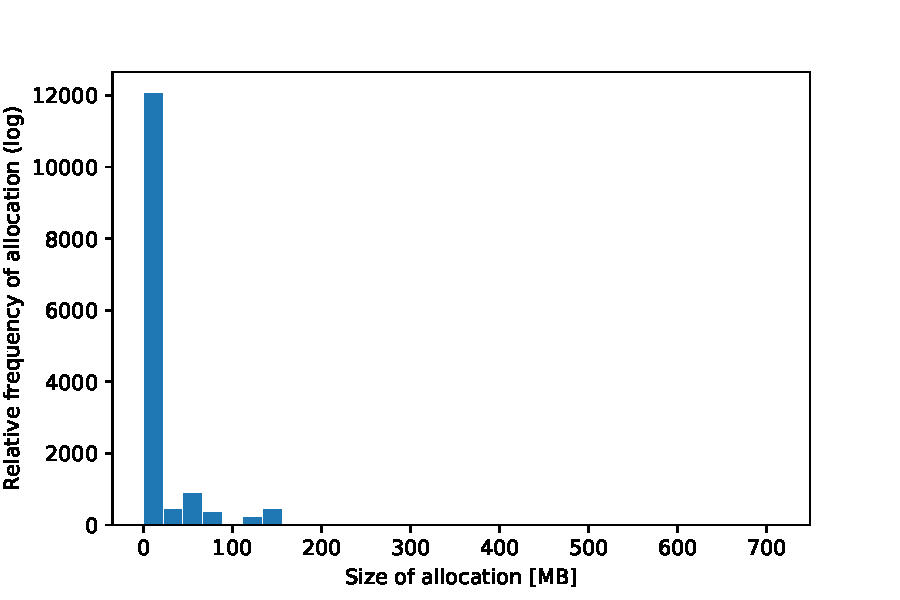
\includegraphics[width=0.5\textwidth]{"../Quantitative Python/histogram.pdf"}
\end{figure}

Initial tests have shown that profiling GPU accelerated sessions in TensorFlow takes a lot of compute time. Compiling TensorFlow takes about two hours on the workstation that is used for benchmarking. The full benchmark as it is run on the website of TensorFlow cannot be run on the NVIDIA K1100M GPU, as it will run out of memory. Decreasing the batch size from 32 to 16 fixes this problem.

The \texttt{ResNet-50} benchmark in its standard form (with batch size 16) takes about 5.5 minutes to run. The full benchmark runs 110 iterations including the warm-up. To run only a single iteration using the NVIDIA Visual Profiler takes 17 hours. It is therefore not feasible to run the full benchmark (with 110 iterations) with the Visual Profiler. However profiling a single iteration provides enough insight in the memory allocation pattern for further analysis.

\section{Discussion}
\label{sec:discussion}
xxxxx xxxx xxxx 

\bibliography{II2202-report}
%%\bibliographystyle{IEEEtran}
\bibliographystyle{myIEEEtran}
\appendix
\section{Insensible Approximation}

Note that the Appendix or Appendices are Optional.


\end{document}
